	\section{Introduction}


    \begin{frame}{Introducing myself}
        \begin{columns}
            % Column 1
            \begin{column}{0.5\textwidth}
                \begin{itemize}
                    \item Isak Hammer, 27 year old, Lofoten
                    \item Graduate student in Industrial Mathematics
                    \item Research Focus: Analysis and numerical techniques for Partial Differential Equations (PDEs), with a strong emphasis on applications for Finite Element Methods (FEM).
                \end{itemize}
            \end{column}

            % Column 2
            \begin{column}{0.5\textwidth}
                \begin{figure}
                    \centering
                    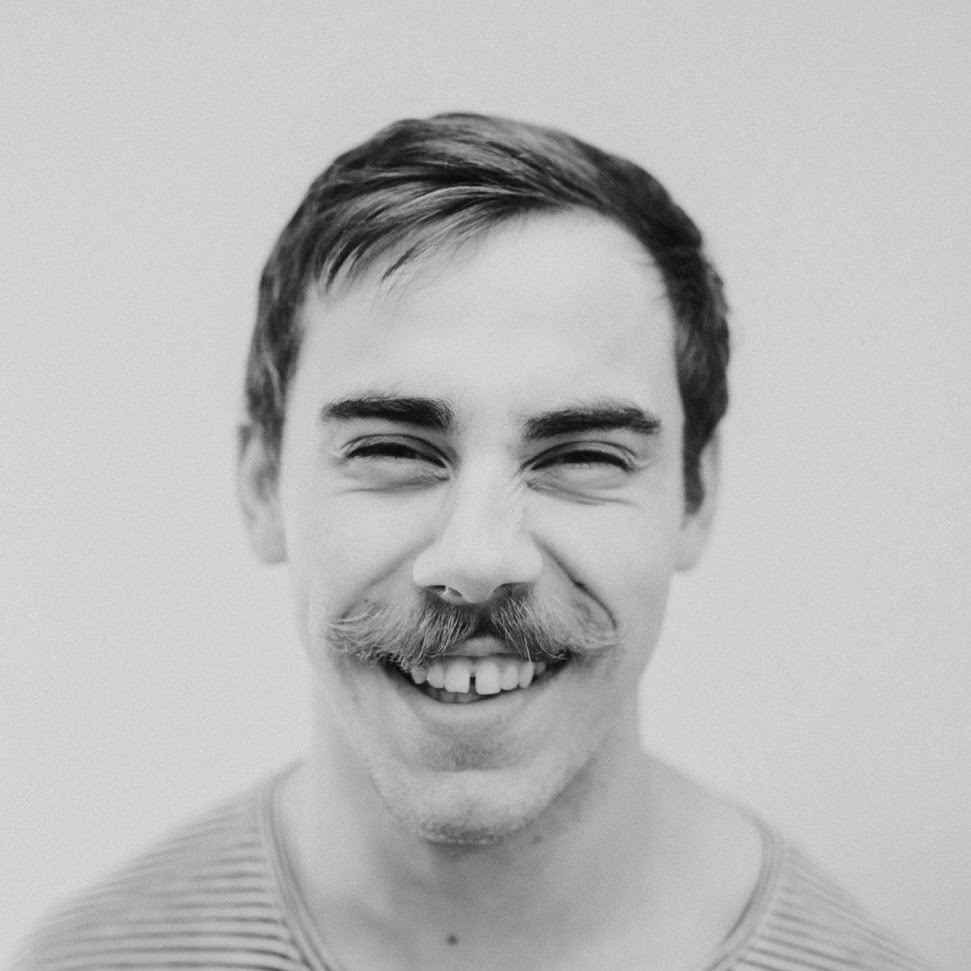
\includegraphics[width=0.7\textwidth]{figures/isak.jpg}
                \end{figure}
            \end{column}
        \end{columns}
    \end{frame}

\begin{frame}{Importance and Motivation of the Cahn Hilliard Equation}
    \begin{columns}
        % Column 1
        \begin{column}{0.5\textwidth}
            \begin{itemize}
            \item Thermodynamically modelling of a two-component liquid separation\footnotemark.
                \item Modelling of so-called lipid rafts in biological membrane dynamics \footnotemark.
            \end{itemize}
        \end{column}
        \begin{column}{0.5\textwidth}
            \begin{itemize}
                \item Droplet dynamics, i.e., coalescence, breakup and movement by coupling with Navier-Stokes \footnotemark.
            \end{itemize}
        \end{column}
    \end{columns}
    \footnotetext[1]{\fullcite{cahn1959free}}
    \footnotetext[2]{\fullcite{yushutin2019computational}}
    \footnotetext[3]{\fullcite{zimmermann2019calculation}}
\end{frame}

\begin{frame}
    \begin{block}{The Cahn Hilliard Equation}
        The general Cahn Hilliard Equation  has the form $u( t,x): \Omega \mapsto [-1,1]   $ s.t.
            \[
            \begin{split}
                 u_t+\Delta\left(\varepsilon \Delta u-\frac{1}{\varepsilon} f(u)\right)&=0 \quad \text{in } \Omega_T:=\Omega \times(0, T) \\
\partial_n u=\partial_n \Delta u& =0 \quad \text{on } \partial \Omega_T:=\partial \Omega \times(0, T) \\
 u & =u_0 \quad \text{on } \Omega \times\{0\}
            \end{split}
            \]
where $f(s)=F^{\prime}(s)$ and $F(s)=\frac{1}{4}\left(s^2-1\right)^2$ and $\Omega \subset \mathbf{R}^d, d=2,3$, is a bounded domain. $\partial_n$ denotes the normal derivative operator on $\partial \Omega$.
\end{block}

\begin{block}{Challenges}
    \begin{enumerate}
        \item Highly nonlinear and stiff. Often practical applications require $\varepsilon \ll 1$.
        \item 4th order system.
        \item Conservation of mass and the Neumann conditions conditions.
    \end{enumerate}
\end{block}

\end{frame}

\begin{frame}
    \begin{block}{Why Finite Element Method (FEM)}
        \begin{enumerate}
            \item \textbf{Flexibility:} Weak formulation provides versatility in imposing boundary conditions effectively.
            \item \textbf{Complex geometries:} FEM can efficiently handle intricate geometries, making it suitable for a wide range of applications.
            \item \textbf{Polynomial basis:} FEM is built upon polynomial basis functions, offering flexibility, accuracy and smoothness in the solution.
            \item \textbf{Other: } Elegant mathematical formulation, supports adaptive refinements, easily adaptable to multi-physics problems, among other benefits.
        \end{enumerate}
    \end{block}
\end{frame}

\begin{frame}
    \begin{block}{Continuous Interior Penalty (CIP) Method}
    \end{block}
\end{frame}


\begin{frame}
    \begin{block}{Illustration of an discontinuous polynomial space}
        \begin{figure}
            \centering
            \begin{minipage}[b]{0.45\textwidth}
                \centering
                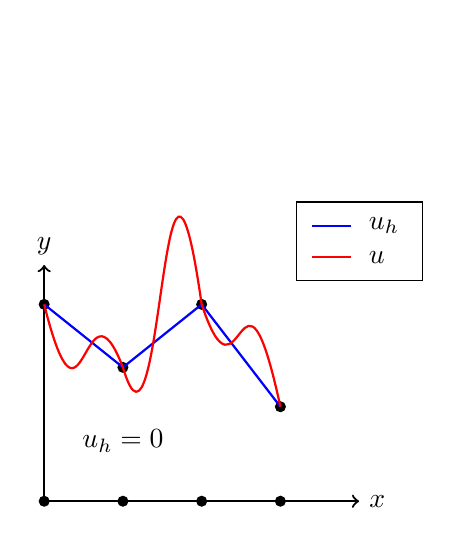
\begin{tikzpicture}
                    % Draw x-axis
                    \draw[->, thick] (0,0) -- (4,0) node[right] {$x$};
                    % Draw y-axis
                    \draw[->, thick] (0,0) -- (0,3) node[above] {$y$};

                    % Draw nodes at center, A, B, and C with arbitrary y-values
                    \foreach \x/\y in {0/2.5, 1/1.7, 2/2.5, 3/1.2} {
                        \fill (\x,\y) circle (2pt); % Filled nodes with y-values
                        \fill (\x,0) circle (2pt); % Filled circles on x-axis
                    }

                    % Draw linear interpolation between points
                    \draw[blue, thick] (0,2.5) -- (1,1.7) -- (2,2.5) -- (3,1.2);

                    \draw[red, thick] (0,2.5) .. controls (0.5,0.5) and (0.5,3) .. (1,1.7) .. controls (1.5,0) and (1.5,6) .. (2,2.5) .. controls (2.5,1) and (2.5,3.5) .. (3,1.2);
                    \node at (1,0.5) [above] {$\jump{ u_{h} } = 0$};

                    \draw (3.2,2.8) rectangle (4.8,3.8); % Legend box
                    \draw[blue, thick] (3.4,3.5) -- (3.9,3.5); % Blue line for u_h
                    \draw[red, thick] (3.4,3.1) -- (3.9,3.1); % Red line for u
                    \node[anchor=west] at (4.0,3.5) {$u_h$}; % Label for u_h
                    \node[anchor=west] at (4.0,3.1) {$u$}; % Label for u

                \end{tikzpicture}
                \caption{Illustration of global $C^{0}$ continuous elements using $P^{1}$.}
                \label{fig:CG_P1_ements}
            \end{minipage}
            \hfill
            \begin{minipage}[b]{0.45\textwidth}
                \centering
                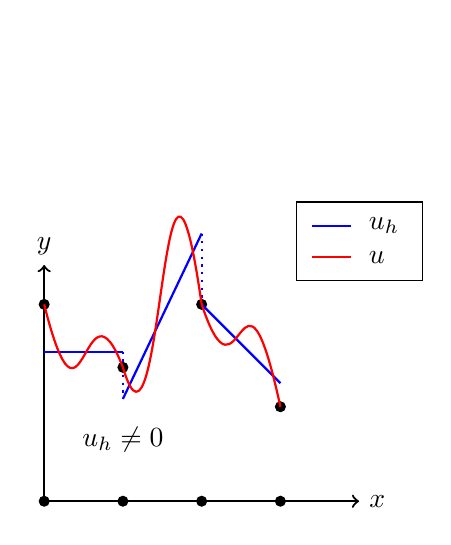
\begin{tikzpicture}
                    % Draw x-axis
                    \draw[->, thick] (0,0) -- (4,0) node[right] {$x$};
                    % Draw y-axis
                    \draw[->, thick] (0,0) -- (0,3) node[above] {$y$};

                    % Draw nodes at center, A, B, and C with arbitrary y-values
                    \foreach \x/\y in {0/2.5, 1/1.7, 2/2.5, 3/1.2} {
                        \fill (\x,\y) circle (2pt); % Filled nodes with y-values
                        \fill (\x,0) circle (2pt); % Filled circles on x-axis
                    }

                    % Draw discontinuous interpolation between points
                    \draw[blue, thick] (0,1.9) -- (1,1.9);
                    \draw[blue, thick] (1,1.3) -- (2,3.4);
                    \draw[blue, thick] (2,2.5) -- (3,1.5);

                    % Draw dotted lines between discontinuous interpolations
                    \draw[blue, thick, dotted] (1,1.9) -- (1,1.3);
                    \draw[blue, thick, dotted] (2,3.4) -- (2,2.5);

                    \node at (1,0.5) [above] {$\jump{ u_{h} } \neq 0$};

                    \draw[red, thick] (0,2.5) .. controls (0.5,0.5) and (0.5,3) .. (1,1.7) .. controls (1.5,0) and (1.5,6) .. (2,2.5) .. controls (2.5,1) and (2.5,3.5) .. (3,1.2);

                    \draw (3.2,2.8) rectangle (4.8,3.8); % Legend box
                    \draw[blue, thick] (3.4,3.5) -- (3.9,3.5); % Blue line for u_h
                    \draw[red, thick] (3.4,3.1) -- (3.9,3.1); % Red line for u
                    \node[anchor=west] at (4.0,3.5) {$u_h$}; % Label for u_h
                    \node[anchor=west] at (4.0,3.1) {$u$}; % Label for u

                \end{tikzpicture}
                \caption{Illustration of locally discontinuous elements using $P^{1}$.}
                \label{fig:DG_P1_ements}
            \end{minipage}
        \end{figure}

    \end{block}
\end{frame}

\begin{frame}
\begin{figure}
  \centering
  \begin{minipage}[b]{0.45\textwidth}
    \centering
    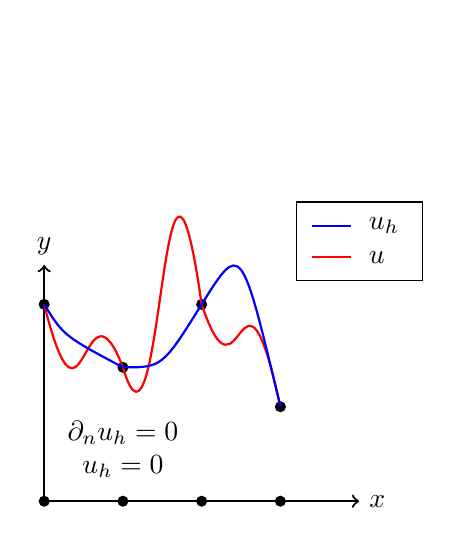
\begin{tikzpicture}
        % Draw x-axis
        \draw[->, thick] (0,0) -- (4,0) node[right] {$x$};
        % Draw y-axis
        \draw[->, thick] (0,0) -- (0,3) node[above] {$y$};

        % Draw nodes at center, A, B, and C with arbitrary y-values
        \foreach \x/\y in {0/2.5, 1/1.7, 2/2.5, 3/1.2} {
            \fill (\x,\y) circle (2pt); % Filled nodes with y-values
            \fill (\x,0) circle (2pt); % Filled circles on x-axis
        }

        % Exact solution
        \draw[red, thick] (0,2.5) .. controls (0.5,0.5) and (0.5,3) .. (1,1.7) .. controls (1.5,0) and (1.5,6) .. (2,2.5) .. controls (2.5,1) and (2.5,3.5) .. (3,1.2);
        \node at (1,0.6) [above] {$\jump{ \partial _{n} u_{h} } = 0$};
        \node at (1,0.7) [below] {$\jump{ u_{h} }   = 0$};

        % Second
        \draw[blue, thick]
        (0,2.5) .. controls (0.25,2.1) .. (1,1.7)
        (1,1.7) .. controls (1.5,1.7) .. (2,2.5)
        (2,2.5) .. controls (2.5,3.3) .. (3,1.2);

        \draw (3.2,2.8) rectangle (4.8,3.8); % Legend box
        \draw[blue, thick] (3.4,3.5) -- (3.9,3.5); % Blue line for u_h
        \draw[red, thick] (3.4,3.1) -- (3.9,3.1); % Red line for u
        \node[anchor=west] at (4.0,3.5) {$u_h$}; % Label for u_h
        \node[anchor=west] at (4.0,3.1) {$u$}; % Label for u

    \end{tikzpicture}
    \caption{Illustration of globally $C^{1}$ continuous elements using $P^{2}$ elements.}
    \label{fig:C1_P2_ements}
  \end{minipage}
  \hfill
  \begin{minipage}[b]{0.45\textwidth}
    \centering
    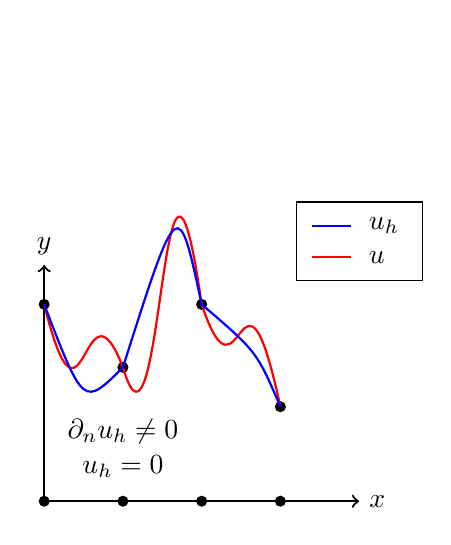
\begin{tikzpicture}
        % Draw x-axis
        \draw[->, thick] (0,0) -- (4,0) node[right] {$x$};
        % Draw y-axis
        \draw[->, thick] (0,0) -- (0,3) node[above] {$y$};

        % Draw nodes at center, A, B, and C with arbitrary y-values
        \foreach \x/\y in {0/2.5, 1/1.7, 2/2.5, 3/1.2} {
            \fill (\x,\y) circle (2pt); % Filled nodes with y-values
            \fill (\x,0) circle (2pt); % Filled circles on x-axis
        }

        % Exact solution
        \draw[red, thick] (0,2.5) .. controls (0.5,0.5) and (0.5,3) .. (1,1.7) .. controls (1.5,0) and (1.5,6) .. (2,2.5) .. controls (2.5,1) and (2.5,3.5) .. (3,1.2);
        \node at (1,0.6) [above] {$\jump{ \partial _{n} u_{h} } \neq 0$};
        \node at (1,0.7) [below] {$\jump{ u_{h} }   = 0$};

        %% Second
        \draw[blue, thick] (0,2.5) .. controls (0.5,1.2) .. (1,1.7)
        .. controls (1.7,3.9) .. (2,2.5)
        .. controls (2.7,1.9) .. (3,1.2); Second

        \draw (3.2,2.8) rectangle (4.8,3.8); % Legend box
        \draw[blue, thick] (3.4,3.5) -- (3.9,3.5); % Blue line for u_h
        \draw[red, thick] (3.4,3.1) -- (3.9,3.1); % Red line for u
        \node[anchor=west] at (4.0,3.5) {$u_h$}; % Label for u_h
        \node[anchor=west] at (4.0,3.1) {$u$}; % Label for u

    \end{tikzpicture}
    \caption{Illustration of $C^{0}$ continuous elements and locally $C^1$ using $P^{2}$.}
    \label{fig:C0_P2_ements}
  \end{minipage}
\end{figure}
\end{frame}


\begin{frame}

\begin{block}{Unfitted mesh vs fitted mesh}
    CutFEM is a numerical method for solving partial differential equations (PDEs) using an unfitted mesh.

\begin{figure}
    \centering
    % First TikZ picture
    \begin{minipage}{0.45\textwidth}
        \centering
        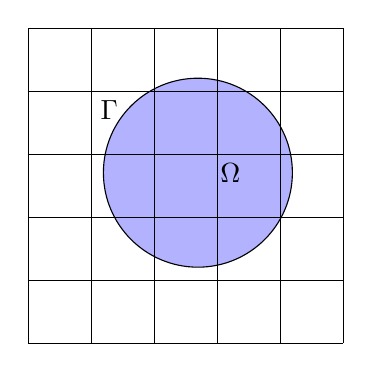
\begin{tikzpicture}[scale=0.80]
            \draw[fill=blue!30] (0.2, 0.2) circle (1.5cm);
            % Background mesh
            \foreach \i in {-2.5, -1.5, ..., 2.5} {
                \draw[line width=0.1pt, shift={(-2.5,\i)}] (0,0) -- (5,0);
                \draw[line width=0.1pt, shift={(\i,-2.5)}] (0,0) -- (0,5);
            }
            % Labels
            \node[below right] at (0.4,0.5) {$\Omega $};
            \node[below right] at (-1.5,1.5) {$\Gamma $};
            % \draw[blue, thick] (-2.5, -2.5) rectangle (2.5, 2.5);
        \end{tikzpicture}
    \end{minipage}
    \hfill
    % Second TikZ picture
    \begin{minipage}{0.45\textwidth}
        \centering
        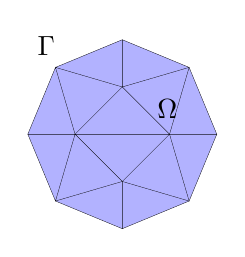
\begin{tikzpicture}[scale=0.80]
            % FIGURE OF UNFITTED MESH
            % Boundary points
            \foreach \i in {0, 45, ..., 315} {
                \coordinate (boundary-\i) at (\i:1.5cm);
            }
            % Interior points
            \coordinate (interior-1) at (0.75, 0);
            \coordinate (interior-2) at (-0.75, 0);
            \coordinate (interior-3) at (0, 0.75);
            \coordinate (interior-4) at (0, -0.75);

            % Create a cycle connecting all the boundary points
            \fill[blue!30] (boundary-0) -- (boundary-45) -- (boundary-90) -- (boundary-135) -- (boundary-180) -- (boundary-225) -- (boundary-270) -- (boundary-315) -- cycle;

            % Labels
            \node[below right] at (0.4,0.7) {$\Omega $};
            \node[below right] at (-1.5,1.7) {$\Gamma $};

            % Triangulation (manually specified)
            \draw[line width=0.1pt] (boundary-0) -- (boundary-45) -- (interior-1) -- cycle;
            \draw[line width=0.1pt] (boundary-45) -- (boundary-90) -- (interior-3) -- cycle;
            \draw[line width=0.1pt] (boundary-90) -- (boundary-135) -- (interior-3) -- cycle;
            \draw[line width=0.1pt] (boundary-135) -- (boundary-180) -- (interior-2) -- cycle;
            \draw[line width=0.1pt] (boundary-180) -- (boundary-225) -- (interior-2) -- cycle;
            \draw[line width=0.1pt] (boundary-225) -- (boundary-270) -- (interior-4) -- cycle;
            \draw[line width=0.1pt] (boundary-270) -- (boundary-315) -- (interior-4) -- cycle;
            \draw[line width=0.1pt] (boundary-315) -- (boundary-0) -- (interior-1) -- cycle;

            % Triangulation between interior points
            \draw[line width=0.1pt] (interior-1) -- (interior-2) -- (interior-3) -- cycle;
            \draw[line width=0.1pt] (interior-1) -- (interior-2) -- (interior-4) -- cycle;

            % \draw[blue, thick] (-2.5, -2.5) rectangle (2.5, 2.5);

        \end{tikzpicture}
    \end{minipage}


    \caption{Mesh comparison: unfitted mesh (left) adheres to domain and boundary, while fitted mesh (right) employs a triangular mesh for polygonal approximation of the circular domain.}
    \label{fig:domain_mesh}
    \end{figure}
\end{block}

\end{frame}

